\subsection{3.1配分函数和分布函数}
我们的第一项任务是讨论理想链模型的配分函数和分布函数是如何在外场存在的情况下进行修改的。我们从离散高斯链开始。
\subsubsection{3.1.1离散高斯链}
主要感兴趣的外场是一个空间变化的化学势场$w(\mathrm{r})$,它作用于离散高斯链的$N+1$个珠子上,我们再次采用图2.1和2.3节的表示法。势能可以写成
\begin{equation}
\begin{aligned}
U(\mathrm{r}^{N+1})&=U_0(\mathrm{r}^{N+1})+U_1(\mathrm{r}^{N+1})\\
&=\sum\limits_{i=1}^Nh(\left|\mathrm{r}_i-\mathrm{r}_{i-1}\right|)+k_BT\sum\limits_{i=0}^Nw(\mathrm{r}_i)
\end{aligned}
\end{equation}
这里$h(x)=3k_BTx^2/(2b^2)$和$\mathrm{r}^{N+1}$是$N+1$个珠子坐标$(\mathrm{r}_0,\mathrm{r}_1,\cdots,\mathrm{r}_N)$的缩写。$N$键上的第一个和是$U_0$,这是离散高斯链的调和伸缩能(harmonic stretching energy)。$N+1$微球上的第二个和计算了每个珠子与势场$k_BTw(\mathrm{r})$的相互作用能。另一种表示外部势能项$U_1(\mathrm{r}^{N+1})$的方法是
\begin{equation}
\beta U_1(\mathrm{r}^{N+1})=\int\mathrm{d}\mathrm{r}w(\mathrm{r})\hat{\rho}(\mathrm{r})
\end{equation}
其中段的微观密度由下式定义:
\begin{equation}
\hat{\rho}(\mathrm{r})=\sum\limits_{i=0}^N\delta(\mathrm{r}-\mathrm{r}_i)
\end{equation}
这种微观密度显然是$\mathrm{r}$的非常奇异的函数,并且显然地依赖于珠子坐标$\mathrm{r}^{N+1}$。式子(3.2)表示的事实是,势场$w(\mathrm{r})$可以看作是一个空间变化的化学势场,它是热力学共轭于段密度的化学势场(Chandler,1987)。

特别令人感兴趣的是,受外部势场$w(\mathrm{r})$,$Z[w]$作用的链的配分函数与理想链的配分函数$Z_0$的比率。
\begin{equation}
Q(w)\equiv\frac{Z[w]}{Z_0}=\frac{\int\mathrm{d}\mathrm{r}^{N+1}\exp[-\beta U(\mathrm{r}^{N+1})]}{V(\int\mathrm{d}\mathbf{b}\exp[-\beta h(\left|\mathbf{b}\right|)])^N}
\end{equation}
在该表达式的分母中,使用了(2.27)式,它将$Z_0$表示为键向量上的体积$V$乘以$N$个独立(体积)积分,如符号所示,归一化配分函数$Q[w]$可以看作是外部势场$w(r)$的函数。

下一步是将等式(3.4)的分母中的$\int\mathrm{d}\mathbf{b}\exp[-\beta h(\left|\mathbf{b}\right|)]$的$N$个因子与分子中的$\exp[-\beta h(\left|\mathrm{r}_i-\mathrm{r}_{i-1}\right|)]$的$N$个因子相关联。回顾离散高斯链的归一化键转移概率的定义,式子(2.34)
\begin{equation}
\Phi(\mathrm{r})=\frac{\exp[-\beta h(\left|\mathrm{r}\right|)]}{\int\mathrm{d}\mathrm{r}\exp[-\beta h(\left|\mathrm{r}\right|)]}=\left(\frac{3}{2\pi b^2}\right)^{3/2}\exp\left(-\frac{3\left|\mathrm{r}\right|^2}{2b^2}\right)
\end{equation}
使等式(3.4)重写为
\begin{equation}
\begin{aligned}
Q[w]=\frac{1}{V}\int\mathrm{d}\mathrm{r}^{N+1}&[e^{-w(\mathrm{r}_N)}\Phi(\mathrm{r}_N-\mathrm{r}_{N-1})e^{-w(\mathrm{r}_{N-1})}\Phi(\mathrm{r}_{N-1}-\mathrm{r}_{N-2})\\
&\cdots e^{-w(\mathrm{r}_2)}\Phi(\mathrm{r}_2-\mathrm{r}_1)e^{-w(\mathrm{r}_1)}\Phi(\mathrm{r}_1-\mathrm{r}_0)e^{-w(\mathrm{r}_0)}]
\end{aligned}
\end{equation}
这个表达式可以按以下方式递归构建。我们对整数$j$定义了一个泛函$q(\mathrm{r},j;[w])$通过
\begin{equation}
q(\mathrm{r},0;[w])=\exp[-w(\mathrm{r})]
\end{equation}
和对$j=0,1,2,\cdots,N-1$
\begin{equation}
q(\mathrm{r},j+1;[w])=\exp[-w(\mathrm{r})]\int\mathrm{d}\mathrm{r}'\Phi(\mathrm{r}-\mathrm{r}')q(\mathrm{r}',j;[w]))
\end{equation}
因此,归一化的配分函数可以表示为
\begin{equation}
Q[w]=\frac{1}{V}\int\mathrm{d}\mathrm{r}q(\mathrm{r},N;[w])
\end{equation}
在上文中,$q(\mathrm{r},j;[w])$表示$j+1$个珠子链在$r$位置处的统计权重。该对象通常被称为链传播子,是外部势场$w(\mathrm{r})$的函数。式子(3.8)可以看作是一个Chapman-Kolmogorov方程,对于无场情况下概率密度$p_0(\mathrm{r},j)$,它与式子(2.33)严格类似。实际上,除了函数$p_0(\mathrm{r},j)$和$q(\mathrm{r},j;[w])$的不同归一化之外,式子(3.8)对于$w(\mathrm{r})\rightarrow 0$被看作是式子(2.33)。

需要注意的是,对于任何弹簧势$h(x)$,式子(3.7)-(3.9)都是成立的,条件是用适当的形式代替高斯模型式子(3.5)的跃迁概率密度$\Phi(\mathrm{r})$。参见式子(2.40),式子(3.7)-(3.9)适用于式子(2.41)等非线性珠弹簧模型。
\begin{figure}[H]
\centering
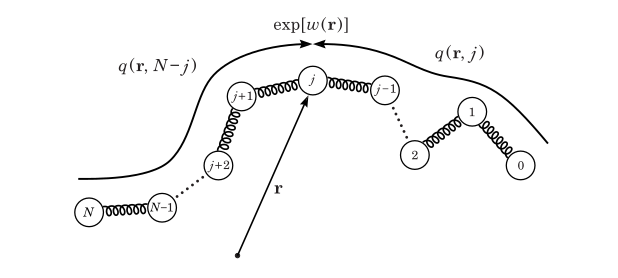
\includegraphics[scale=0.7]{./figures/Figure_1.png}
\caption{因式分解性质eqn(3.10)的物理内容,具有$j+1$珠的传播子可以在第$j$个珠的位置$\mathrm{r}=\mathrm{r}_j$处连接到具有$N-j+1$珠的传播子,以产生链的总统计量。在结点处需要$\exp[w(\mathrm{r})]$的因子。}
\end{figure}
归一化配分函数$Q[w]$具有一个重要的因式分解性质,如图3.1所示。如果我们选择在珠$j$处计算eqn(3.6),那么很明显,$Q[w]$是可以成
\begin{equation}
Q[w]=\frac{1}{V}\int\mathrm{d}\mathrm{r}q(\mathrm{r},N-j;[w])\exp[w(\mathrm{r})]q(\mathrm{r},j;[w])
\end{equation}
这个表达式的物理解释是,通过将链端分布的传播子与$N-j+1$珠子的“互补”链的传播子连接起来,可以建立$(N+1)$珠链的统计权重。传播子在第$j$个珠的位置连接,$\mathrm{r}=\mathrm{r}_j$,并包含$\exp[w(\mathrm{r})]$以抵消与两个连接端相关联的$\exp[-w(\mathrm{r})]$的过量因子。

第二类外势对研究聚合物的力学响应具有重要意义,它是一个应变场。在这里,我们限制了对均匀应变$\epsilon(\mathrm{r})=\epsilon$的关注,以了解这种对称张量场是如何与聚合物的统计力学耦合的,需要注意的是,可以写出离散高斯链弹性应力张量的微观表达式(Doi和Edwards,1986)
\begin{equation}
\hat{\sigma}_{\alpha\gamma}(\mathrm{r})=\frac{3k_BT}{b^2}\sum\limits_{i=1}^N\delta(\mathrm{r}-\mathrm{r}_{i-1})(\mathrm{r}_{i}-\mathrm{r}_{i-1})_{\alpha}(\mathrm{r}_i-\mathrm{r}_{i-1})_{\gamma}
\end{equation}
其中希腊语下标再次用于表示张量的笛卡尔指数,该表达式表示与穿过规定平面的聚合物键相关的每单位面积的弹力。利用应力和应变是共轭热力学变量的事实,(Landu和Lifshitz,1986),可以写出与施加的应变$\epsilon$相关的弹性能量。
\begin{equation}
U_{el}(\mathrm{r}^{N+1})=\int\mathrm{d}\mathrm{r}\epsilon:\hat{\boldsymbol{\sigma}}(\mathrm{r})
\end{equation}
特别令人感兴趣的是配分函数$Z[w,\epsilon]$,一个受化学势场和应变场双重作用的离散高斯链。在这种情况下,最方便的归一化是$w=0$的链的配分函数,但不消失应变
\begin{equation}
Q[w,\epsilon]\equiv\frac{Z[w,\epsilon]}{Z[0,\epsilon]}=\frac{\int\mathrm{d}\mathrm{r}^{N+1}\exp[-\beta U(\mathrm{r}^{N+1})-\beta U_{el}(\mathrm{r}^{N+1})]}{\int\mathrm{d}\mathrm{r}^{N+1}\exp[-\beta U_0(\mathrm{r}^{N+1})-\beta U_{el}(\mathrm{r}^{N+1})]}
\end{equation}
导致eqns(3.7)-(3.9)的论点仍然适用,但随着键转移概率的变化
\begin{equation}
\Psi(\mathrm{r};[\epsilon])=\left(\frac{3}{2\pi b^2}\right)^{3/2}[det(1+2\epsilon)]^{1/2}\exp\left(-\frac{3}{2b^2}(1+2\epsilon:\mathrm{r}\mathrm{r})\right)
\end{equation}
其中$1$表示单位张量。在推导这个表达式时使用了eqn(B.11),在无应变情况下,$Q[w,\epsilon]$可以根据
\begin{equation}
Q[w,\epsilon]=\frac{1}{V}\int\mathrm{d}\mathrm{r}q(\mathrm{r},N;[w,\epsilon])
\end{equation}
计算且
\begin{equation}
q(\mathrm{r},0;[w,\epsilon])=\exp[-w(\mathrm{r})]
\end{equation}
和
\begin{equation}
q(\mathrm{r},j+1;[w,\epsilon])=\exp[-w(\mathrm{r})]\int\mathrm{d}\mathrm{r}'\Psi(\mathrm{r}-\mathrm{r}';[\epsilon])q(\mathrm{r}',j;[w,\epsilon])
\end{equation}
对于$j=0,1,2,\cdots,N-1$。这些方程在消失应变$\epsilon\rightarrow 0$的极限下明显降低到eqn(3.7)-(3.9),在消失应变和化学势$\epsilon,w\rightarrow 0$。
\subsubsection{3.1.2连续高斯链}
前一段的公式可以很容易地推广到连续高斯链模型,微观段密度由eqn(3.3)变为
\begin{equation}
\hat{\rho}(\mathrm{r})=\int_0^N\mathrm{d}s\delta(\mathrm{r}-\mathrm{r}(s))
\end{equation}
与施加的化学势场$w(\mathrm{r})$相关的势能成为聚合物形状$\mathrm{r}(s)$的函数。
\begin{equation}
\beta U_1[\mathrm{r},w]=\int\mathrm{d}\mathrm{r}'w(\mathrm{r}')\hat{\rho}(\mathrm{r}')
\end{equation}
归一化配分函数$Q[w]$可以表示为路径积分的比率。
\begin{equation}
Q[w]\equiv\frac{Z[w]}{Z_0}=\frac{\int\mathcal{D}\mathrm{r}\exp(-\beta U_0[\mathrm{r}]-\beta U_1[\mathrm{r},w])}{\int\mathcal{D}\mathrm{r}\exp(-\beta U_0[\mathrm{r}])}
\end{equation}
在此定义下,$Z_0$的奇点从分子和分母中完全消失,在连续链极限中呈现$Q[w]$有限。利用$N_s+1$珠和$N_s$弹簧,根据equ(2.45)对两个路径积分进行离散化,并对离散高斯链的步骤进行了回溯,得到了eqn(3.6)。因此,eqn(3.20)减少到
\begin{equation}
\begin{aligned}
Q[w]=\frac{1}{V}&\int\mathrm{d}\mathrm{r}^{N_s+1}[e^{-\Delta sw(\mathrm{r}_{N_s})}\Phi(\mathrm{r}_{N_s}-\mathrm{r}_{N_s-1})e^{-\Delta sw(\mathrm{r}_{N_s-1})}\\
&\times\quad\Phi(\mathrm{r}_{N_s-1}-\mathrm{r}_{N_s-2})\cdots e^{-\Delta sw(\mathrm{r}_2)}\\
&\times\quad\Phi(\mathrm{r}_2-\mathrm{r}_1)\cdots e^{-\Delta sw(\mathrm{r}_1)}\Phi(\mathrm{r}_1-\mathrm{r}_0)e^{-\Delta sw(\mathrm{r}_0)}]
\end{aligned}
\end{equation}
其中$\Phi(\mathrm{r}-\mathrm{r}')=\Phi(\Delta\mathrm{r})$由eqn(2.59)和$\Delta s\equiv N/N_s$给出。和以前一样,$Q[w]$的表达式可以写成
\begin{equation}
Q[w]=\frac{1}{V}\int\mathrm{d}\mathrm{r}q(\mathrm{r},N;[w])
\end{equation}
这里
\begin{equation}
q(\mathrm{r},0;[w])=\exp[-\Delta sw(\mathrm{r})]
\end{equation}
和
\begin{equation}
q(\mathrm{r},s+\Delta s;[w])=\exp[-\Delta sw(\mathrm{r})]\int\mathrm{d}\mathrm{r}'\Phi(\mathrm{r}-\mathrm{r}')q(\mathrm{r}',s;[w])
\end{equation}
用于沿着从$s=0$到$s=N$链向前的方向,以$\Delta s$的$N_s$为增量。

方程(3.24)是一个Chapman-Kolmogorov方程,与无场情况下的方程(2.58)密切相关,它可以在$\Delta s\rightarrow 0$的连续极限中转换为Fokker-Planck方程。泰勒展式在$\Delta s$中将eqn(3.24)的两边展开为一阶的,在$\Delta\mathrm{r}=\mathrm{r}-\mathrm{r}'$中将被积函数展开为二阶的,人们发现(Edwards,1965;de Gennes,1969;Freed,1972)
\begin{equation}
\frac{\partial}{\partial s}q(r,s;[w])=\frac{b^2}{6}\nabla^2q(\mathrm{r},s;[w])-w(\mathrm{r})q(\mathrm{r},s;[w])s
\end{equation}
它可以看作是eqn(2.64)的推广,包括外部势场。“初始条件”eqn(3.23)在连续极限下减小到均匀条件。
\begin{equation}
q(\mathrm{r},0;[w])=1
\end{equation}
Fokker-Planck方程(3.25)通常称为修正的扩散方程,有时与量子力学的路径积分公式相似,称为Feynman-Kac公式(Feynman和Hibbs,1965)。结合eqn(3.22),改进的扩散方程充分描述了外部势场$w(\mathrm{r})$中连续高斯链的统计力学。这是非均匀聚合物理论中最重要的结果之一。

势$w(\mathrm{r})$中的连续高斯链具有类似于离散高斯链的eqn(3.10)的因式分解性质。特别是,
\begin{equation}
Q[w]=\frac{1}{V}\int\mathrm{d}\mathrm{r}q(\mathrm{r},N-s;[w])q(\mathrm{r},s;[w])
\end{equation}
其中路径积分已被分解在任意轮廓位置$0<s<N$。由于连续极限在$\Delta s\rightarrow 0$时$\exp[\Delta sw(\mathrm{r})]\rightarrow 0$,因此在连接端消除过量因子$\exp[-\Delta sw(\mathrm{r})]$所需的指数因子$\exp[\Delta sw(\mathrm{r})]$是不存在的。

除了化学势场$w(\mathrm{r})$外,这些结果很容易推广到均匀应变场$\epsilon$作用下的连续高斯链情形。将微观弹性应力表达式(3.11)修正为连续高斯链
\begin{equation}
\hat{\sigma}_{\alpha\gamma}(\mathrm{r})=\frac{3k_BT}{b^2}\int_0^N\mathrm{d}s\delta(\mathrm{r}-\mathrm{r}(s))\frac{\mathrm{d}\mathrm{r}_{\alpha}(s)}{\mathrm{d}s}\frac{\mathrm{d}\mathrm{r}_{\gamma}(s)}{\mathrm{d}s}
\end{equation}
弹性能可以表示为$\mathrm{r}(s)$和$\epsilon$的泛函
\begin{equation}
U_{el}[\mathrm{r},\epsilon]=\int\mathrm{d}\mathrm{r}'\epsilon:\hat{\sigma}(\mathrm{r}')
\end{equation}
对于经历应变和化学势场的连续链的归一化配分函数是
\begin{equation}
Q[w,\epsilon]\equiv\frac{Z[w,\epsilon]}{Z[0,\epsilon]}=\frac{\int\mathcal{D}\mathrm{r}\exp(-\beta U_0[\mathrm{r}]-\beta U_1[\mathrm{r},w]-\beta U_{el}[\mathrm{r},\epsilon])}{\int\mathcal{D}\mathrm{r}\exp(-\beta U_0[\mathrm{r}]-\beta U_{el}[\mathrm{r},\epsilon])}
\end{equation}
再次,归一化是$Q[0,\epsilon]=1$,根据方程(2.45)将分子和分母中的路径积分分离并且回溯导致方程(3.25)的步骤产生以下结果(Fredrickson,2002)
\begin{equation}
Q[w,\epsilon]=\frac{1}{V}\int\mathrm{d}\mathrm{r}q(\mathrm{r},N;[w,\epsilon])
\end{equation}
其中传播子$q(\mathrm{r},s;[w,\epsilon])$满足Fokker-Planck方程。
\begin{equation}
\begin{aligned}
\frac{\partial}{\partial s}q(\mathrm{r},s;[w,\epsilon])=&-w(\mathrm{r})q(\mathrm{r},s;[w,\epsilon])\\
&+\frac{b^2}{6}(1+2\epsilon)^{-1}:\nabla\nabla q(\mathrm{r},s;[w,\epsilon])
\end{aligned}
\end{equation}
这个方程受初始条件的影响。
\begin{equation}
q(\mathrm{r},0;[w,\epsilon])=1
\end{equation}
Fokker-Planck方程(3.32)在消失应变情况下可变为eqn(3.25)。然而,在有限$\epsilon$条件下,它描述了一个各向异性扩散过程,它与同时经历化学势场和应变场的聚合物链相一致。这些结果可进一步推广到非均匀应变场$\epsilon(\mathrm{r})$的情形(Fredrickson,2002)。
\subsubsection{3.1.3虫状链}
类似蠕虫的链模型也可以类似地扩展到包含与外部场的相互作用。与高斯链模型不同的是,蠕虫状链通常用来描述具有局部刚性的聚合物,这些聚合物具有液晶有序性。这种液晶在微观上来源于各向异性的节段相互作用。因此,必须允许目前情况下的外部“化学”势即取决于分段位置,也取决于方向,即$w=w(\mathrm{r},\mathrm{u})$。虫族链与这样一个场的相互作用能可以写成。
\begin{equation}
\begin{aligned}
\beta U_1[\mathrm{r},w]&=\int_0^{L_c}\mathrm{d}sw(\mathrm{r}(s),\mathrm{u}(s))\\
&=\int\mathrm{d}\mathrm{r}'\int\mathrm{d}\mathrm{u}'w(\mathrm{r}',\mathrm{u}')\hat{\rho}(\mathrm{r}',\mathrm{u}')
\end{aligned}
\end{equation}
这里
\begin{equation}
\hat{\rho}(\mathrm{r},\mathrm{u})\equiv\int_0^{L_c}\mathrm{d}s\delta(\mathrm{r}-\mathrm{r}(s))\delta(\mathrm{u}-\mathrm{u}(s))
\end{equation}
是片段位置和取向的微观位置。势$w(\mathrm{r},\mathrm{u})$与这个密度是热力学共轭的。

在无势$Z_0$的情况下,用它的值归一化的蠕虫链的配分函数$w(\mathrm{r},\mathrm{u})$,$Z[w]$可以写成
\begin{equation}
Q[w]\equiv\frac{Z[w]}{Z_0}=\frac{\int^*\mathcal{D}\mathrm{r}\exp(-\beta U_0[\mathrm{u}]-\beta U_1[\mathrm{r},w])}{\int^*\mathcal{D}\mathrm{r}\exp(-\beta U_0[\mathrm{u}])}
\end{equation}
其中$U_0[\mathrm{u}]$是eqn(2.66)中给出的弯曲能。分子和分母中路径积分上的星号是表示equ(2.67)的约束的简记,即
\begin{equation}
\prod\limits_s\delta\left(\mathrm{u}(s)-\frac{\mathrm{d}\mathrm{r}(s)}{\mathrm{d}s}\right)\delta(\left|\mathrm{u}(s)\right|-1)
\end{equation}
是强加于链构相$\mathrm{r}(s)$上的。

方程(3.36)可以通过离散分子和分母中的路径积分和推导链传播子$q(\mathrm{r},\mathrm{u},s;[w])$类似于(2.71)的Chapman-Kolmogorov方程来求解。这个量描述了像蠕虫一样的轮链长度的链,并且位于势场$w(\mathrm{r},\mathrm{u})$,其末端段在位置$\mathrm{r}$和方位$u$的统计权重。归一化配分函数是从
\begin{equation}
Q[w]=\frac{1}{4\pi V}\int\mathrm{d}\mathrm{r}\int\mathrm{d}\mathrm{u}q(\mathrm{r},\mathrm{u},L_c;[w])
\end{equation}
在连续极限中,我们发现类蠕虫链传播子$q(\mathrm{r},\mathrm{u},s;[w])$满足无场情况下类似eqn(2.76)的Fokker-Planck方程:
\begin{equation}
\begin{aligned}
\frac{\partial}{\partial s}q(\mathrm{r},\mathrm{u},s;[w])=&-w(\mathrm{r},\mathrm{u})q(\mathrm{r},\mathrm{u},s;[w])-\mathrm{u}\cdot\nabla_{\mathrm{r}}q(\mathrm{r},\mathrm{u},s;[w])\\
&+\frac{1}{2\lambda}\nabla_{\mathrm{u}}^2q(\mathrm{r},\mathrm{u},s;[w])
\end{aligned}
\end{equation}
这个方程是在初始条件下求解的
\begin{equation}
q(\mathrm{r},\mathrm{u},0;[w])=1
\end{equation}
方程(3.38)-(3.40)是定义具有外部势的蠕虫链的统计力学的基本关系。

类蠕虫链的归一化配分函数具有类似于连续高斯链的因式分解性质。从$Q[w]$的离散表达式可以直接推断出
\begin{equation}
Q[w]=\frac{1}{4\pi V}\int\mathrm{d}\mathbf{r}\int\mathrm{d}\mathbf{u}q(\mathbf{r},-\mathbf{u},L_c-s;[w])q(\mathbf{r},\mathbf{u},s;[w])
\end{equation}
对于任意$0\le s\le L$。在物理上,这个公式表明,对于总轮廓长度$l_c$的聚合物,可以通过将等轮廓长度$s$的链段的传播子与长度为$L_c-s$的链的第二传播子组成一个传播子来建立配分函数。与第一传播子$q(\mathbf{r},\mathbf{u},s;[w])$相关的统计权重是通过从聚合物的$s=0$段开始在eqns(3.39)-(3.40)沿$s$方向向前积分得到的。第二个传播子$q(\mathbf{r},-\mathbf{u},L_c-s;[w])$对应于通过求解eqns(3.39)-(3.40)得到的长度为$L_c-s$的链的统计权重,从另一端开始的聚合物。该权重中的切向量$u$在符号中是反向的,以说明沿链轮廓的传播方向的差异。

虽然我们把$w$称为外化学势场,但所采用的形式$w=w(\mathbf{r},\mathbf{u})$足以描述多种类型的外势,包括电场和磁场。例如,一种感兴趣的情况是沿着主干网具有永久电偶极子的链,它与切线向量$\mathbf{u}(s)$共线,即$\mu(s)=\mu_0\mathbf{u}(s)$。在这种情况下,与施加的静止电场$\mathbf{E}(\mathbf{r})$相关的静电能由eqn(3.34)和
\begin{equation}
w(\mathbf{r},\mathbf{u})=-\beta\mu_0\mathbf{E}(\mathbf{r})\cdot\mathbf{u}
\end{equation}
作为另一个例子,在静电场$\mathbf{E}(\mathbf{r})$作用下,介电虫状链可以用下面势来描述:
\begin{equation}
w(\mathbf{r},\mathbf{u})=-\frac{\beta}{2}\mathbf{E}(\mathbf{r})\cdot\boldsymbol{\alpha}(\mathbf{u})\cdot\mathbf{E}(\mathbf{r})
\end{equation}
其中$\boldsymbol{\alpha}(\mathbf{u})$是取向$\mathbf{u}$的差分链段的极化率张量。在关于$\mathbf{u}$的极化率张量的圆柱对称的特殊情况下,$\boldsymbol{\alpha}(\mathbf{u})$可以表示为
\begin{equation}
\boldsymbol{\alpha}(\mathbf{u})=\alpha_{\parallel}\mathbf{u}\mathbf{u}+\alpha_{\perp}(1-\mathbf{u}\mathbf{u})
\end{equation}
其中,$\alpha_{\parallel}$和$\alpha_{\perp}$分别是差分链段平行和垂直于切线向量$\mathbf{u}$的极化率。

类似的表达式可以用来描述类蠕虫链与一大类静态和时变外场之间的相互作用。我们将对液晶的各向异性势场的讨论推迟到4.6节。

不幸的是,沿着蠕虫状链弯曲的三体特性使微观张力的识别变得复杂。在克服这一困难之前,不可能探索蠕虫状链对空间变化应变场的平衡效应。
\subsubsection{3.1.4棒状聚合物}
类蠕虫链模型具有一种吸引人的特性,即它根据持续长度和轮廓长度的比值$(\lambda/L_c)$,在刚性杆和柔性线圈之间进行连续插补。因此,它可以用来描述任意主干网灵活性的大分子。然而,该模型的一个严重缺点是,在计算热力学和结构量时,需要一个传播子$q(\mathbf{r},\mathbf{u},s)$,它在高斯链模型中传播子$q(\mathbf{r},s)$之外还有两个附加的内部坐标(定义$\mathbf{u}$的角度)。在3.6节中,很明显,这些额外的坐标大大增加了用类蠕虫链模型进行数值计算的费用。因此,对于近柔性聚合物$\lambda/L_c\gg 1$,最好用连续高斯链或珠弹簧链模型代替类蠕虫链。类似地,对于接近刚性的棒状聚合物,$\lambda/L_c\gtrsim 1$,采用严格的棒状聚合物模型代替类蠕虫链。对于一端为$\mathbf{r}$且取向为$\mathbf{u}$的长$L_c$的杆,给出了归一化配分函数如下:
\begin{equation}
Q[w]=\frac{1}{4\pi V}\int\mathrm{d}\mathbf{r}\int\mathrm{d}\mathbf{u}\exp\left[-\int_0^{L_c}\mathrm{d}sw(\mathbf{r}+s\mathbf{u},\mathbf{u})\right]
\end{equation}
给定一定的势场$w(\mathbf{r},\mathbf{u})$,eqn(3.45)比相应的eqns(3.38)-(3.40)更直观。










































































































